\documentclass{book}
\usepackage[utf8]{inputenc}
\usepackage{polski}
\usepackage[polish]{babel}
\usepackage{setspace}
\usepackage{graphicx}
\usepackage{listings}

\onehalfspacing

% According to polish grammar rules, you have to put dots after numerals in chapter, section, subsection, etc. headers.
\renewcommand\thechapter{\arabic{chapter}.}
\renewcommand\thesection{\arabic{chapter}.\arabic{section}.}
\renewcommand\thesubsection{\arabic{chapter}.\arabic{section}.\arabic{subsection}.}
\renewcommand\thesubsubsection{\arabic{chapter}.\arabic{section}.\arabic{subsection}.%
                                                           \arabic{subsubsection}.}
% It's customary (depends on publisher) to indent first paragraph in sections and chapters:
\usepackage{indentfirst}

\begin{document}

\chapter{Shell interaktywny}
% TODO Topics covered

Zanim rozpoczniemy pisać gry komputerowe, powinniśmy poznać kilka pojęć związanych z programowaniem. Chodzi o wartości, operatory, wyrażenia i zmienne. Nie zaczniemy w tym rozdziale programować, ale poznanie tych pojęć i różnych nazw bardzo uprości naukę programowania. To dlatego, że większa część programowania to tylko kilka prostych pomysłów połączonych w całość i tworzących duże programy.

Zacznijmy od nauczenia się jak używać interaktywnego shella Pythona.

\section{Trochę prostej matematyki}

Żeby otworzyć IDLE na Windowsie, kliknij na Start, Programy, Python 3.1 a potem IDLE (Python GUI). Zaczniemy od kilku prostych obliczeń w Pythonie. Interaktywny shell może działać jak kalkulator. Wpisz w okno shella 2+2 i wciśnij Enter na klawiaturze (na niektórych klawiaturach ten klawisz to Return). Jak widzisz na rysunku~\ref{idle-dwaplusdwa}, komputer powinien odpowiedzieć liczbą 4, sumą 2+2.

\begin{figure}
\centerline{
%	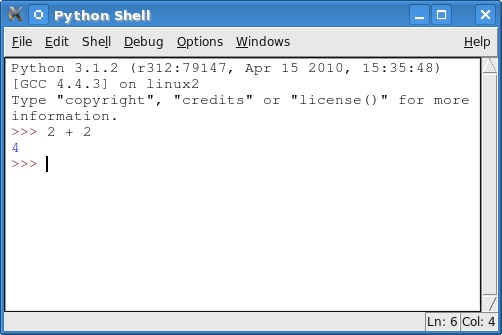
\includegraphics[width=2cm]{idle-dwaplusdwa.png}
}
\caption{Wpisz w okno shella 2+2}
\label{idle-dwaplusdwa}
\end{figure}

Jak widzisz, możemy używać shella Pythona jak kalkulatora. To nie jest jeszcze program ponieważ w tej chwili uczymy się dopiero podstaw. Znak + każe komputerowi dodać liczby 2 i 2. Aby udjąć liczby, użyj znaku -, żeby je pomnożyć użyj gwiazdki (*), w ten sposób:

\begin{table}[here]
\caption{Różne operatory matematyczne w Pythonie}
\centerline{
\begin{tabular}{| c | c | }
\hline
2+2 & dodawanie\\
\hline
2-2 & odejmowanie\\
\hline
2*2 & mnożenie\\
\hline
2/2 & dzielenie\\
\hline
\end{tabular}
}
\label{hops-algo}
\end{table}

Znaki +, -, * i / kiedy używa się ich w ten sposób, są nazywane {\bf operatorami} ponieważ mówią komputerowi żeby wykonał jakąś operację na liczbach które je otaczają.

\subsection{Liczby całkowite i zmiennoprzecinkowe}

W programowaniu (a także matematyce), liczby takie jak 4, 0 czy 99 nazywane są {\bf całkowitymi}. Liczby z ułamkami bądź kropką dziesiętną\footnote{W matematyce do oddzielania części całkowitej od ułamkowej używa się przecinka, w programowaniu - zazwyczaj jest to kropka.} (jak 3.5, 42.1, 5.0) nie są całkowite. W Pythonie, liczba 5 jest całkowita, ale jeśli zapiszemy ją jako 5.0 - już nie. Liczby z kropką dziesiętną nazywają się {\bf liczbami zmiennoprzecinkowymi}. W matematyce, 5.0 ciągle pozostaje liczbą całkowitą i taką samą liczbą jak 5, ale w programowaniu - komputer nie traktuje liczb z kropką dziesiątną jako całkowitych.

\subsection{Wyrażenia}

Spróbuj wpisać któreś z tych działań do shella, wciskając po każdym z nich Enter.

\lstset{language=python}
\begin{lstlisting}{}
2+2+2+2+2
8*6
10-5+6
2  +       2
\end{lstlisting}

\begin{figure}
\centerline{
%	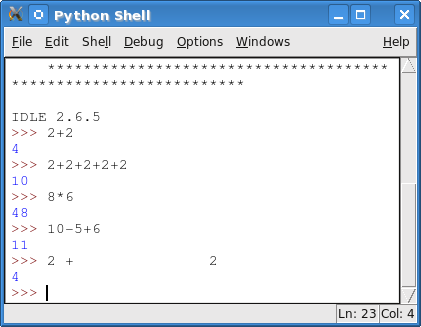
\includegraphics[width=2cm]{idle-wyrazenia.png}
}
\caption{Okno IDLE po wykonaniu wyrażeń}
\label{idle-dwaplusdwa}
\end{figure}

% TODO rysunek o wyrażeniu
Te działania matematyczne nazywane są wyrażeniami. Komputery potrafią rozwiązać miliony tego typu zadań w ciągu sekundy. Wyrażenia są złożone z {\bf wartości} (liczb) połączonych {\bf operatorami} (symbolami matematycznymi). Dowiedzmy się czym dokładnie są wartości i operatory.

%TODO straszliwie są napisane te dwa akapity
Jak widzisz w ostatnim wyrażeniu w powyższym przykładzie, możesz użyć dowolnej ilości spacji pomiędzy liczbami a operatorami (ale pamiętaj żeby zawsze zaczynać od samego początku linii, bez spacji na początku).

Liczba jest rodzajem wartości. Liczba całkowita jest rodzajem liczby. Ale, chociaż liczby całkowite są liczbami, nie wszystkie liczby są liczbami całkowitymi (na przykład, ułamki i liczby z kropką dziesiętną jak 2.5 są liczbami ale nie są całkowite).

To podobnie jak kot jest rodzajem zwierzęcia domowego, ale nie wszystkie zwierzęta domowe są kotami. Są przecież ludzie którzy mają psy lub kraby. {\bf Wyrażenie} składa się z wartości (na przykład liczb całkowitych takich jak 8 czy 6) połączonych operatorem (takim jak znak mnożenia *). Pojedyńcza wartość bez operatorów też traktowana jest jak wyrażenie.

W następnym rozdziale nauczymy się jak pracować z wyrażeniami tekstowymi. Python nie jest ograniczony do liczb. Umie wiele więcej niż zwykły kalkulator.

\section{Ewaluacja wyrażeń}

Kiedy komputer rozwiązuje wyrażenie 10+5 i otrzymuje wartość 15, mówimy że {\bf ewaluuje\footnote{oblicza}} wyrażenie. Ewaluacja wyrażenia redukuje je do pojedynczej wartości, podobnie jak rozwiązanie zadania matematycznego redukuje zadanie do pojedynczej liczby: rozwiązania.

Wyrażenia 10+5 oraz 10+3+2 mają tą samą wartość, ponieważ oba są ewaluowane do 15. Nawet pojedyncze wartości są wyrażeniami: wyrażenie 15 ewaluuje się do wartośći 15.

Jeśli jednak wpiszesz w interaktywnym shellu tylko 5+, dostaniesz wiadomość o błędzie.
\lstset{language=python}
\begin{lstlisting}{}
>>> 5 +
SyntaxError: invalid syntax
\end{lstlisting}



\end{document}
